\documentclass{whiteboard}
\begin{document}
\begin{frame}[plain,t]
\bbcover{Grafos}{Componentes fortemente conectados}{Prof. Edson Alves}{Faculdade UnB Gama}

\end{frame}
\begin{frame}[plain,t]
\begin{tikzpicture}
\node[draw,opacity=0] at (0, 0) {x};
\node[draw,opacity=0] at (14, 8) {x};

	\node[anchor=west] (title) at (0.0, 6.5) { \Large \bbbold{Grafos fortemente conectados} };
\end{tikzpicture}
\end{frame}
\begin{frame}[plain,t]
\begin{tikzpicture}
\node[draw,opacity=0] at (0, 0) {x};
\node[draw,opacity=0] at (14, 8) {x};

	\node[anchor=west] (title) at (0.0, 6.5) { \Large \bbbold{Grafos fortemente conectados} };

	\node[anchor=west] (a) at (1.0, 5.5) { \bbtext{Seja $G(V, E)$ um grafo direcionado. Dizemos que $G$ é \bbbold{fortemente conectado}} };

	\node[anchor=west] (a1) at (0.5, 4.75) { \bbtext{se, para qualquer par de vértices $u, v\in V$, existe pelo menos um caminho de} };

	\node[anchor=west] (a2) at (0.5, 4.0) { \bbtext{$u$ até $v$.} };

\end{tikzpicture}
\end{frame}
\begin{frame}[plain,t]
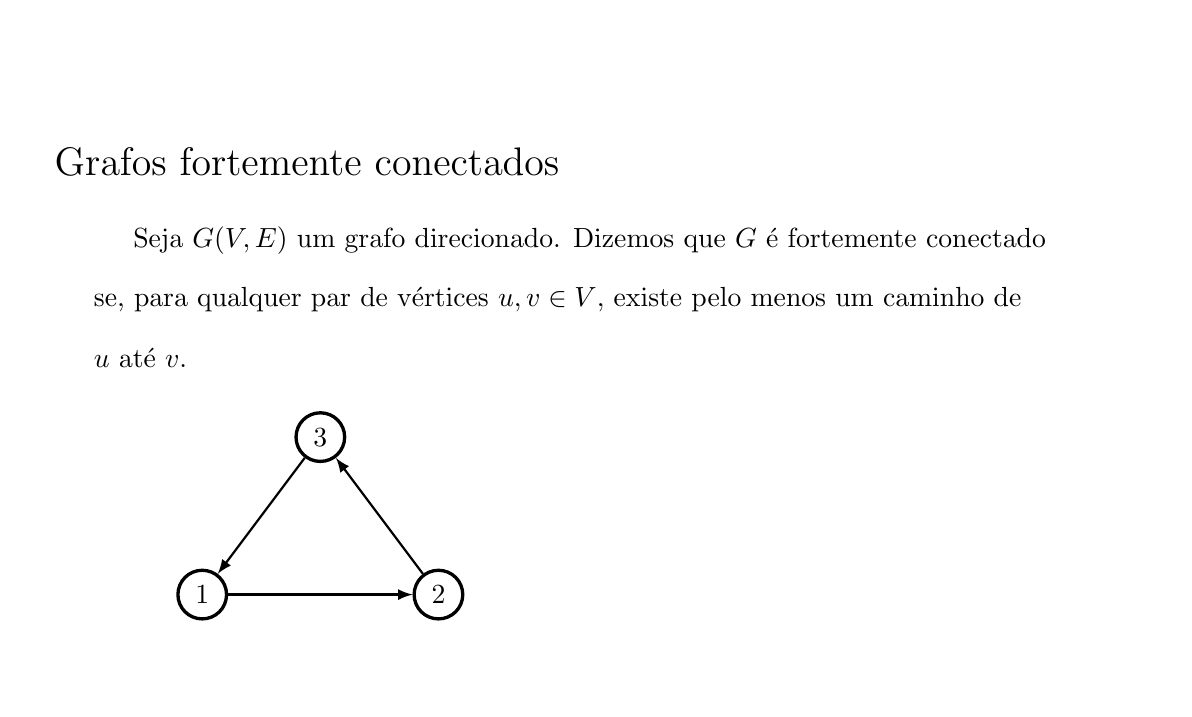
\begin{tikzpicture}
\node[draw,opacity=0] at (0, 0) {x};
\node[draw,opacity=0] at (14, 8) {x};

	\node[anchor=west] (title) at (0.0, 6.5) { \Large \bbbold{Grafos fortemente conectados} };

	\node[anchor=west] (a) at (1.0, 5.5) { \bbtext{Seja $G(V, E)$ um grafo direcionado. Dizemos que $G$ é \bbbold{fortemente conectado}} };

	\node[anchor=west] (a1) at (0.5, 4.75) { \bbtext{se, para qualquer par de vértices $u, v\in V$, existe pelo menos um caminho de} };

	\node[anchor=west] (a2) at (0.5, 4.0) { \bbtext{$u$ até $v$.} };


	\node[very thick,draw,circle] (node1) at (2.0, 1.0) { \bbtext{1} };

	\node[very thick,draw,circle] (node2) at (5.0, 1.0) { \bbtext{2} };

	\node[very thick,draw,circle] (node3) at (3.5, 3.0) { \bbtext{3} };

	\draw[thick,-latex](node1) to (node2);

	\draw[thick,-latex](node2) to (node3);

	\draw[thick,-latex](node3) to (node1);

\end{tikzpicture}
\end{frame}
\begin{frame}[plain,t]
\begin{tikzpicture}
\node[draw,opacity=0] at (0, 0) {x};
\node[draw,opacity=0] at (14, 8) {x};

	\node[anchor=west] (title) at (0.0, 6.5) { \Large \bbbold{Grafos fortemente conectados} };

	\node[anchor=west] (a) at (1.0, 5.5) { \bbtext{Seja $G(V, E)$ um grafo direcionado. Dizemos que $G$ é \bbbold{fortemente conectado}} };

	\node[anchor=west] (a1) at (0.5, 4.75) { \bbtext{se, para qualquer par de vértices $u, v\in V$, existe pelo menos um caminho de} };

	\node[anchor=west] (a2) at (0.5, 4.0) { \bbtext{$u$ até $v$.} };


	\node[very thick,draw,circle] (node1) at (2.0, 1.0) { \bbtext{1} };

	\node[very thick,draw,circle] (node2) at (5.0, 1.0) { \bbtext{2} };

	\node[very thick,draw,circle] (node3) at (3.5, 3.0) { \bbtext{3} };

	\draw[thick,-latex](node1) to (node2);

	\draw[thick,-latex](node2) to (node3);

	\draw[thick,-latex](node3) to (node1);


	\node[anchor=west] (text1) at (5.5, 2.5) { \bbtext{\Large \textcolor{BBGreen}{\faCheck}} };

\end{tikzpicture}
\end{frame}
\begin{frame}[plain,t]
\begin{tikzpicture}
\node[draw,opacity=0] at (0, 0) {x};
\node[draw,opacity=0] at (14, 8) {x};

	\node[anchor=west] (title) at (0.0, 6.5) { \Large \bbbold{Grafos fortemente conectados} };

	\node[anchor=west] (a) at (1.0, 5.5) { \bbtext{Seja $G(V, E)$ um grafo direcionado. Dizemos que $G$ é \bbbold{fortemente conectado}} };

	\node[anchor=west] (a1) at (0.5, 4.75) { \bbtext{se, para qualquer par de vértices $u, v\in V$, existe pelo menos um caminho de} };

	\node[anchor=west] (a2) at (0.5, 4.0) { \bbtext{$u$ até $v$.} };


	\node[very thick,draw,circle] (node1) at (2.0, 1.0) { \bbtext{1} };

	\node[very thick,draw,circle] (node2) at (5.0, 1.0) { \bbtext{2} };

	\node[very thick,draw,circle] (node3) at (3.5, 3.0) { \bbtext{3} };

	\draw[thick,-latex](node1) to (node2);

	\draw[thick,-latex](node2) to (node3);

	\draw[thick,-latex](node3) to (node1);


	\node[anchor=west] (text1) at (5.5, 2.5) { \bbtext{\Large \textcolor{BBGreen}{\faCheck}} };


	\node[very thick,draw,circle] (node4) at (8.0, 1.0) { \bbtext{4} };

	\node[very thick,draw,circle] (node5) at (11.0, 1.0) { \bbtext{5} };

	\node[very thick,draw,circle] (node6) at (9.5, 3.0) { \bbtext{6} };

	\draw[thick,-latex](node4) to (node5);

	\draw[thick,-latex](node4) to (node6);


	\draw[thick,-latex](node5) to (node6);


\end{tikzpicture}
\end{frame}
\begin{frame}[plain,t]
\begin{tikzpicture}
\node[draw,opacity=0] at (0, 0) {x};
\node[draw,opacity=0] at (14, 8) {x};

	\node[anchor=west] (title) at (0.0, 6.5) { \Large \bbbold{Grafos fortemente conectados} };

	\node[anchor=west] (a) at (1.0, 5.5) { \bbtext{Seja $G(V, E)$ um grafo direcionado. Dizemos que $G$ é \bbbold{fortemente conectado}} };

	\node[anchor=west] (a1) at (0.5, 4.75) { \bbtext{se, para qualquer par de vértices $u, v\in V$, existe pelo menos um caminho de} };

	\node[anchor=west] (a2) at (0.5, 4.0) { \bbtext{$u$ até $v$.} };


	\node[very thick,draw,circle] (node1) at (2.0, 1.0) { \bbtext{1} };

	\node[very thick,draw,circle] (node2) at (5.0, 1.0) { \bbtext{2} };

	\node[very thick,draw,circle] (node3) at (3.5, 3.0) { \bbtext{3} };

	\draw[thick,-latex](node1) to (node2);

	\draw[thick,-latex](node2) to (node3);

	\draw[thick,-latex](node3) to (node1);


	\node[anchor=west] (text1) at (5.5, 2.5) { \bbtext{\Large \textcolor{BBGreen}{\faCheck}} };


	\node[very thick,draw,circle] (node4) at (8.0, 1.0) { \bbtext{4} };

	\node[very thick,draw,circle] (node5) at (11.0, 1.0) { \bbtext{5} };

	\node[very thick,draw,circle] (node6) at (9.5, 3.0) { \bbtext{6} };

	\draw[thick,-latex](node4) to (node5);

	\draw[thick,-latex](node4) to (node6);


	\draw[thick,-latex](node5) to (node6);



	\node[anchor=west] (text2) at (11.5, 2.5) { \bbtext{\Large \textcolor{BBRed}{\faClose}} };


\end{tikzpicture}
\end{frame}
\begin{frame}[plain,t]
\begin{tikzpicture}
\node[draw,opacity=0] at (0, 0) {x};
\node[draw,opacity=0] at (14, 8) {x};

	\node[anchor=west] (title) at (0.0, 6.5) { \Large \bbbold{Componentes fortemente conectados} };
\end{tikzpicture}
\end{frame}
\begin{frame}[plain,t]
\begin{tikzpicture}
\node[draw,opacity=0] at (0, 0) {x};
\node[draw,opacity=0] at (14, 8) {x};

	\node[anchor=west] (title) at (0.0, 6.5) { \Large \bbbold{Componentes fortemente conectados} };

	\node[anchor=west] (a) at (1.0, 5.5) { \bbtext{Seja $G(V, E)$ um grafo direcionado. Um \bbbold{componente fortemente conectado}} };

	\node[anchor=west] (b) at (0.5, 4.75) { \bbtext{ de $G$ é um subgrafo $S$ de $G$ fortemente conectado.} };

\end{tikzpicture}
\end{frame}
\begin{frame}[plain,t]
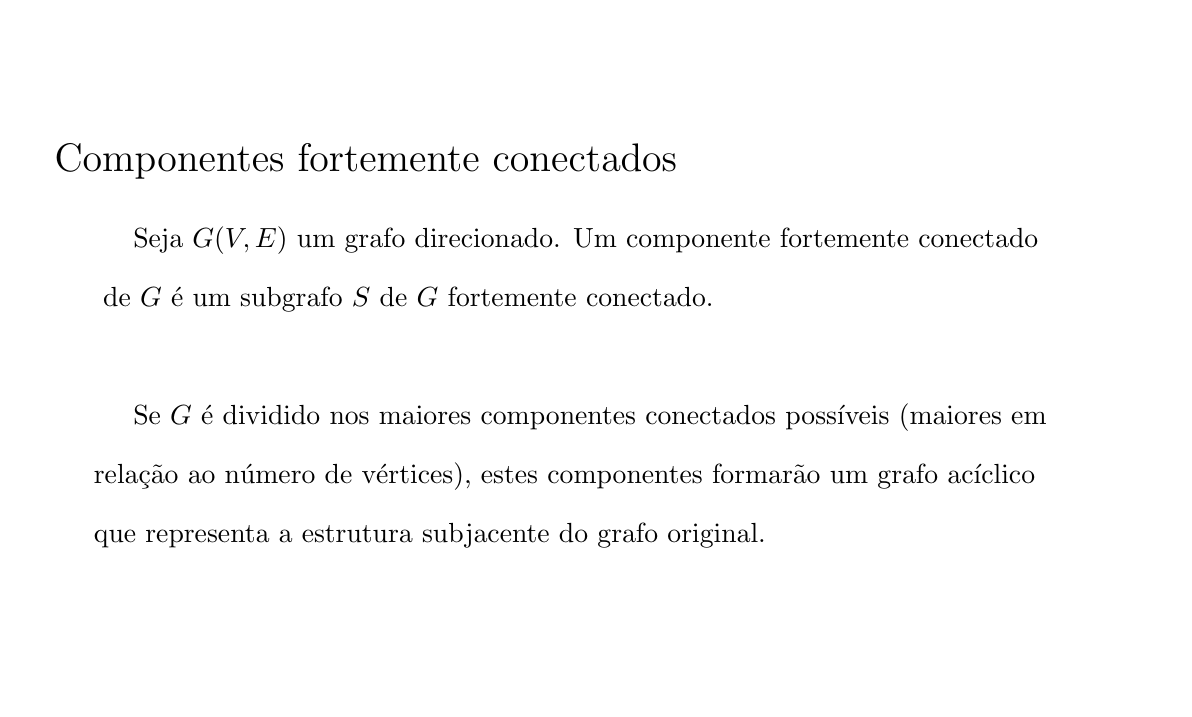
\begin{tikzpicture}
\node[draw,opacity=0] at (0, 0) {x};
\node[draw,opacity=0] at (14, 8) {x};

	\node[anchor=west] (title) at (0.0, 6.5) { \Large \bbbold{Componentes fortemente conectados} };

	\node[anchor=west] (a) at (1.0, 5.5) { \bbtext{Seja $G(V, E)$ um grafo direcionado. Um \bbbold{componente fortemente conectado}} };

	\node[anchor=west] (b) at (0.5, 4.75) { \bbtext{ de $G$ é um subgrafo $S$ de $G$ fortemente conectado.} };


	\node[anchor=west] (b1) at (1.0, 3.25) { \bbtext{Se $G$ é dividido nos maiores componentes conectados possíveis (maiores em} };

	\node[anchor=west] (b2) at (0.5, 2.5) { \bbtext{relação ao número de vértices), estes componentes formarão um grafo acíclico} };

	\node[anchor=west] (c) at (0.5, 1.75) { \bbtext{que representa a estrutura subjacente do grafo original.} };

\end{tikzpicture}
\end{frame}
\begin{frame}[plain,t]
\begin{tikzpicture}
\node[draw,opacity=0] at (0, 0) {x};
\node[draw,opacity=0] at (14, 8) {x};

	\node[very thick,draw,circle] (node1) at (1.0, 4.0) { \bbtext{1} };

	\node[very thick,draw,circle] (node2) at (4.0, 6.0) { \bbtext{2} };

	\node[very thick,draw,circle] (node3) at (4.0, 2.0) { \bbtext{3} };

	\node[very thick,draw,circle] (node4) at (7.0, 6.0) { \bbtext{4} };

	\node[very thick,draw,circle] (node5) at (7.0, 2.0) { \bbtext{5} };

	\node[very thick,draw,circle] (node7) at (10.0, 6.0) { \bbtext{7} };

	\node[very thick,draw,circle] (node6) at (10.0, 2.0) { \bbtext{6} };

	\node[very thick,draw,circle] (node8) at (13.0, 4.0) { \bbtext{8} };

	\draw[thick,-latex](node1) to (node2);

	\draw[thick,-latex](node1) to (node3);

	\draw[thick,-latex](node3) to [bend right] (node2);

	\draw[thick,-latex](node2) to [bend right] (node3);

	\draw[thick,-latex](node2) to (node4);

	\draw[thick,-latex](node3) to (node4);

	\draw[thick,-latex](node4) to (node5);

	\draw[thick,-latex](node4) to (node7);

	\draw[thick,-latex](node5) to (node6);

	\draw[thick,-latex](node6) to (node7);

	\draw[thick,-latex](node6) to (node8);

	\draw[thick,-latex](node7) to (node5);

	\draw[thick,-latex](node8) to (node7);

\end{tikzpicture}
\end{frame}
\begin{frame}[plain,t]
\begin{tikzpicture}
\node[draw,opacity=0] at (0, 0) {x};
\node[draw,opacity=0] at (14, 8) {x};

	\node[very thick,draw,circle,fill=BBCyan] (node1) at (1.0, 4.0) { \bbtext{1} };

	\node[very thick,draw,circle] (node2) at (4.0, 6.0) { \bbtext{2} };

	\node[very thick,draw,circle] (node3) at (4.0, 2.0) { \bbtext{3} };

	\node[very thick,draw,circle] (node4) at (7.0, 6.0) { \bbtext{4} };

	\node[very thick,draw,circle] (node5) at (7.0, 2.0) { \bbtext{5} };

	\node[very thick,draw,circle] (node7) at (10.0, 6.0) { \bbtext{7} };

	\node[very thick,draw,circle] (node6) at (10.0, 2.0) { \bbtext{6} };

	\node[very thick,draw,circle] (node8) at (13.0, 4.0) { \bbtext{8} };

	\draw[thick,-latex](node1) to (node2);

	\draw[thick,-latex](node1) to (node3);

	\draw[thick,-latex](node3) to [bend right] (node2);

	\draw[thick,-latex](node2) to [bend right] (node3);

	\draw[thick,-latex](node2) to (node4);

	\draw[thick,-latex](node3) to (node4);

	\draw[thick,-latex](node4) to (node5);

	\draw[thick,-latex](node4) to (node7);

	\draw[thick,-latex](node5) to (node6);

	\draw[thick,-latex](node6) to (node7);

	\draw[thick,-latex](node6) to (node8);

	\draw[thick,-latex](node7) to (node5);

	\draw[thick,-latex](node8) to (node7);


	\draw[color=BBRed,dashed] (0.25, 3.25) -- (0.25, 4.75) -- (1.75, 4.75) -- (1.75, 3.25) -- cycle;

\end{tikzpicture}
\end{frame}
\begin{frame}[plain,t]
\begin{tikzpicture}
\node[draw,opacity=0] at (0, 0) {x};
\node[draw,opacity=0] at (14, 8) {x};

	\node[very thick,draw,circle,fill=BBCyan] (node1) at (1.0, 4.0) { \bbtext{1} };

	\node[very thick,draw,circle,fill=BBGreen] (node2) at (4.0, 6.0) { \bbtext{2} };

	\node[very thick,draw,circle,fill=BBGreen] (node3) at (4.0, 2.0) { \bbtext{3} };

	\node[very thick,draw,circle] (node4) at (7.0, 6.0) { \bbtext{4} };

	\node[very thick,draw,circle] (node5) at (7.0, 2.0) { \bbtext{5} };

	\node[very thick,draw,circle] (node7) at (10.0, 6.0) { \bbtext{7} };

	\node[very thick,draw,circle] (node6) at (10.0, 2.0) { \bbtext{6} };

	\node[very thick,draw,circle] (node8) at (13.0, 4.0) { \bbtext{8} };

	\draw[thick,-latex](node1) to (node2);

	\draw[thick,-latex](node1) to (node3);

	\draw[thick,-latex](node3) to [bend right] (node2);

	\draw[thick,-latex](node2) to [bend right] (node3);

	\draw[thick,-latex](node2) to (node4);

	\draw[thick,-latex](node3) to (node4);

	\draw[thick,-latex](node4) to (node5);

	\draw[thick,-latex](node4) to (node7);

	\draw[thick,-latex](node5) to (node6);

	\draw[thick,-latex](node6) to (node7);

	\draw[thick,-latex](node6) to (node8);

	\draw[thick,-latex](node7) to (node5);

	\draw[thick,-latex](node8) to (node7);


	\draw[color=BBRed,dashed] (0.25, 3.25) -- (0.25, 4.75) -- (1.75, 4.75) -- (1.75, 3.25) -- cycle;


	\draw[color=BBRed,dashed] (3.25, 1.25) -- (3.25, 6.75) -- (4.75, 6.75) -- (4.75, 1.25) -- cycle;

\end{tikzpicture}
\end{frame}
\begin{frame}[plain,t]
\begin{tikzpicture}
\node[draw,opacity=0] at (0, 0) {x};
\node[draw,opacity=0] at (14, 8) {x};

	\node[very thick,draw,circle,fill=BBCyan] (node1) at (1.0, 4.0) { \bbtext{1} };

	\node[very thick,draw,circle,fill=BBGreen] (node2) at (4.0, 6.0) { \bbtext{2} };

	\node[very thick,draw,circle,fill=BBGreen] (node3) at (4.0, 2.0) { \bbtext{3} };

	\node[very thick,draw,circle,fill=BBViolet] (node4) at (7.0, 6.0) { \bbtext{4} };

	\node[very thick,draw,circle] (node5) at (7.0, 2.0) { \bbtext{5} };

	\node[very thick,draw,circle] (node7) at (10.0, 6.0) { \bbtext{7} };

	\node[very thick,draw,circle] (node6) at (10.0, 2.0) { \bbtext{6} };

	\node[very thick,draw,circle] (node8) at (13.0, 4.0) { \bbtext{8} };

	\draw[thick,-latex](node1) to (node2);

	\draw[thick,-latex](node1) to (node3);

	\draw[thick,-latex](node3) to [bend right] (node2);

	\draw[thick,-latex](node2) to [bend right] (node3);

	\draw[thick,-latex](node2) to (node4);

	\draw[thick,-latex](node3) to (node4);

	\draw[thick,-latex](node4) to (node5);

	\draw[thick,-latex](node4) to (node7);

	\draw[thick,-latex](node5) to (node6);

	\draw[thick,-latex](node6) to (node7);

	\draw[thick,-latex](node6) to (node8);

	\draw[thick,-latex](node7) to (node5);

	\draw[thick,-latex](node8) to (node7);


	\draw[color=BBRed,dashed] (0.25, 3.25) -- (0.25, 4.75) -- (1.75, 4.75) -- (1.75, 3.25) -- cycle;


	\draw[color=BBRed,dashed] (3.25, 1.25) -- (3.25, 6.75) -- (4.75, 6.75) -- (4.75, 1.25) -- cycle;


	\draw[color=BBRed,dashed] (6.25, 5.25) -- (6.25, 6.75) -- (7.75, 6.75) -- (7.75, 5.25) -- cycle;

\end{tikzpicture}
\end{frame}
\begin{frame}[plain,t]
\begin{tikzpicture}
\node[draw,opacity=0] at (0, 0) {x};
\node[draw,opacity=0] at (14, 8) {x};

	\node[very thick,draw,circle,fill=BBCyan] (node1) at (1.0, 4.0) { \bbtext{1} };

	\node[very thick,draw,circle,fill=BBGreen] (node2) at (4.0, 6.0) { \bbtext{2} };

	\node[very thick,draw,circle,fill=BBGreen] (node3) at (4.0, 2.0) { \bbtext{3} };

	\node[very thick,draw,circle,fill=BBViolet] (node4) at (7.0, 6.0) { \bbtext{4} };

	\node[very thick,draw,circle,fill=BBOrange] (node5) at (7.0, 2.0) { \bbtext{5} };

	\node[very thick,draw,circle,fill=BBOrange] (node7) at (10.0, 6.0) { \bbtext{7} };

	\node[very thick,draw,circle,fill=BBOrange] (node6) at (10.0, 2.0) { \bbtext{6} };

	\node[very thick,draw,circle,fill=BBOrange] (node8) at (13.0, 4.0) { \bbtext{8} };

	\draw[thick,-latex](node1) to (node2);

	\draw[thick,-latex](node1) to (node3);

	\draw[thick,-latex](node3) to [bend right] (node2);

	\draw[thick,-latex](node2) to [bend right] (node3);

	\draw[thick,-latex](node2) to (node4);

	\draw[thick,-latex](node3) to (node4);

	\draw[thick,-latex](node4) to (node5);

	\draw[thick,-latex](node4) to (node7);

	\draw[thick,-latex](node5) to (node6);

	\draw[thick,-latex](node6) to (node7);

	\draw[thick,-latex](node6) to (node8);

	\draw[thick,-latex](node7) to (node5);

	\draw[thick,-latex](node8) to (node7);


	\draw[color=BBRed,dashed] (0.25, 3.25) -- (0.25, 4.75) -- (1.75, 4.75) -- (1.75, 3.25) -- cycle;


	\draw[color=BBRed,dashed] (3.25, 1.25) -- (3.25, 6.75) -- (4.75, 6.75) -- (4.75, 1.25) -- cycle;


	\draw[color=BBRed,dashed] (6.25, 5.25) -- (6.25, 6.75) -- (7.75, 6.75) -- (7.75, 5.25) -- cycle;


	\draw[color=BBRed,dashed] (6.25, 1.25) -- (6.25, 2.75) -- (9.25, 6.75) -- (10.75, 6.75) -- (13.75, 4.75) -- (13.75, 3.25) -- (10.75, 1.25) -- cycle;

\end{tikzpicture}
\end{frame}
\begin{frame}[plain,t]
\begin{tikzpicture}
\node[draw,opacity=0] at (0, 0) {x};
\node[draw,opacity=0] at (14, 8) {x};

	\node[very thick,draw,circle,fill=BBCyan] (node1) at (1.0, 4.0) { {\Huge \bbbold{A}} };

	\node[very thick,draw,circle,fill=BBGreen] (node2) at (4.0, 6.0) { \bbtext{2} };

	\node[very thick,draw,circle,fill=BBGreen] (node3) at (4.0, 2.0) { \bbtext{3} };

	\node[very thick,draw,circle,fill=BBViolet] (node4) at (7.0, 6.0) { \bbtext{4} };

	\node[very thick,draw,circle,fill=BBOrange] (node5) at (7.0, 2.0) { \bbtext{5} };

	\node[very thick,draw,circle,fill=BBOrange] (node7) at (10.0, 6.0) { \bbtext{7} };

	\node[very thick,draw,circle,fill=BBOrange] (node6) at (10.0, 2.0) { \bbtext{6} };

	\node[very thick,draw,circle,fill=BBOrange] (node8) at (13.0, 4.0) { \bbtext{8} };

	\draw[thick,-latex](node1) to (node2);

	\draw[thick,-latex](node1) to (node3);

	\draw[thick,-latex](node3) to [bend right] (node2);

	\draw[thick,-latex](node2) to [bend right] (node3);

	\draw[thick,-latex](node2) to (node4);

	\draw[thick,-latex](node3) to (node4);

	\draw[thick,-latex](node4) to (node5);

	\draw[thick,-latex](node4) to (node7);

	\draw[thick,-latex](node5) to (node6);

	\draw[thick,-latex](node6) to (node7);

	\draw[thick,-latex](node6) to (node8);

	\draw[thick,-latex](node7) to (node5);

	\draw[thick,-latex](node8) to (node7);




	\draw[color=BBRed,dashed] (3.25, 1.25) -- (3.25, 6.75) -- (4.75, 6.75) -- (4.75, 1.25) -- cycle;


	\draw[color=BBRed,dashed] (6.25, 5.25) -- (6.25, 6.75) -- (7.75, 6.75) -- (7.75, 5.25) -- cycle;


	\draw[color=BBRed,dashed] (6.25, 1.25) -- (6.25, 2.75) -- (9.25, 6.75) -- (10.75, 6.75) -- (13.75, 4.75) -- (13.75, 3.25) -- (10.75, 1.25) -- cycle;


\end{tikzpicture}
\end{frame}
\begin{frame}[plain,t]
\begin{tikzpicture}
\node[draw,opacity=0] at (0, 0) {x};
\node[draw,opacity=0] at (14, 8) {x};

	\node[very thick,draw,circle,fill=BBCyan] (node1) at (1.0, 4.0) { {\Huge \bbbold{A}} };

	\node[very thick,draw,circle,fill=BBGreen] (node2) at (4.0, 6.0) { {\Huge \bbbold{B}} };


	\node[very thick,draw,circle,fill=BBViolet] (node4) at (7.0, 6.0) { \bbtext{4} };

	\node[very thick,draw,circle,fill=BBOrange] (node5) at (7.0, 2.0) { \bbtext{5} };

	\node[very thick,draw,circle,fill=BBOrange] (node7) at (10.0, 6.0) { \bbtext{7} };

	\node[very thick,draw,circle,fill=BBOrange] (node6) at (10.0, 2.0) { \bbtext{6} };

	\node[very thick,draw,circle,fill=BBOrange] (node8) at (13.0, 4.0) { \bbtext{8} };

	\draw[thick,-latex](node1) to (node2);




	\draw[thick,-latex](node2) to (node4);


	\draw[thick,-latex](node4) to (node5);

	\draw[thick,-latex](node4) to (node7);

	\draw[thick,-latex](node5) to (node6);

	\draw[thick,-latex](node6) to (node7);

	\draw[thick,-latex](node6) to (node8);

	\draw[thick,-latex](node7) to (node5);

	\draw[thick,-latex](node8) to (node7);






	\draw[color=BBRed,dashed] (6.25, 5.25) -- (6.25, 6.75) -- (7.75, 6.75) -- (7.75, 5.25) -- cycle;


	\draw[color=BBRed,dashed] (6.25, 1.25) -- (6.25, 2.75) -- (9.25, 6.75) -- (10.75, 6.75) -- (13.75, 4.75) -- (13.75, 3.25) -- (10.75, 1.25) -- cycle;



\end{tikzpicture}
\end{frame}
\begin{frame}[plain,t]
\begin{tikzpicture}
\node[draw,opacity=0] at (0, 0) {x};
\node[draw,opacity=0] at (14, 8) {x};

	\node[very thick,draw,circle,fill=BBCyan] (node1) at (1.0, 4.0) { {\Huge \bbbold{A}} };

	\node[very thick,draw,circle,fill=BBGreen] (node2) at (4.0, 6.0) { {\Huge \bbbold{B}} };


	\node[very thick,draw,circle,fill=BBViolet] (node4) at (7.0, 6.0) { {\Huge \bbbold{C}} };

	\node[very thick,draw,circle,fill=BBOrange] (node5) at (7.0, 2.0) { \bbtext{5} };

	\node[very thick,draw,circle,fill=BBOrange] (node7) at (10.0, 6.0) { \bbtext{7} };

	\node[very thick,draw,circle,fill=BBOrange] (node6) at (10.0, 2.0) { \bbtext{6} };

	\node[very thick,draw,circle,fill=BBOrange] (node8) at (13.0, 4.0) { \bbtext{8} };

	\draw[thick,-latex](node1) to (node2);




	\draw[thick,-latex](node2) to (node4);


	\draw[thick,-latex](node4) to (node5);

	\draw[thick,-latex](node4) to (node7);

	\draw[thick,-latex](node5) to (node6);

	\draw[thick,-latex](node6) to (node7);

	\draw[thick,-latex](node6) to (node8);

	\draw[thick,-latex](node7) to (node5);

	\draw[thick,-latex](node8) to (node7);








	\draw[color=BBRed,dashed] (6.25, 1.25) -- (6.25, 2.75) -- (9.25, 6.75) -- (10.75, 6.75) -- (13.75, 4.75) -- (13.75, 3.25) -- (10.75, 1.25) -- cycle;




\end{tikzpicture}
\end{frame}
\begin{frame}[plain,t]
\begin{tikzpicture}
\node[draw,opacity=0] at (0, 0) {x};
\node[draw,opacity=0] at (14, 8) {x};

	\node[very thick,draw,circle,fill=BBCyan] (node1) at (1.0, 4.0) { {\Huge \bbbold{A}} };

	\node[very thick,draw,circle,fill=BBGreen] (node2) at (4.0, 6.0) { {\Huge \bbbold{B}} };


	\node[very thick,draw,circle,fill=BBViolet] (node4) at (7.0, 6.0) { {\Huge \bbbold{C}} };



	\node[very thick,draw,circle,fill=BBOrange] (node6) at (10.0, 2.0) { {\Huge \bbbold{D}} };


	\draw[thick,-latex](node1) to (node2);




	\draw[thick,-latex](node2) to (node4);





















	\draw[thick,-latex](node4) to (node6);

\end{tikzpicture}
\end{frame}
\begin{frame}[plain,t]
\begin{tikzpicture}
\node[draw,opacity=0] at (0, 0) {x};
\node[draw,opacity=0] at (14, 8) {x};

	\node[anchor=west] (title) at (0.0, 6.0) { \Large \bbbold{Referências} };

	\node[anchor=west] (b) at (1.0, 5.0) { $1.$ \bbbold{HALIM}, \bbtext{Felix}; \bbbold{HALIM}, \bbtext{Steve}. \bbenglish{Competitive Programming 3,} \bbtext{2010.} };

	\node[anchor=west] (c) at (1.0, 4.0) { $2.$ \bbbold{LAAKSONEN}, \bbtext{Antti}. \bbenglish{Competitive Programmer's Handbook,} \bbtext{2018.} };

\end{tikzpicture}
\end{frame}
\end{document}
